\let\negmedspace\undefined
\let\negthickspace\undefined
\documentclass[journal]{IEEEtran}
\usepackage[a5paper, margin=10mm, onecolumn]{geometry}
\usepackage{lmodern} % Ensure lmodern is loaded for pdflatex
\usepackage{tfrupee} % Include tfrupee package

\setlength{\headheight}{1cm} % Set the height of the header box
\setlength{\headsep}{0mm}     % Set the distance between the header box and the top of the text

\usepackage{gvv-book}
\usepackage{gvv}
\usepackage{cite}
\usepackage{amsmath,amssymb,amsfonts,amsthm}
\usepackage{algorithmic}
\usepackage{graphicx}
\usepackage{textcomp}
\usepackage{xcolor}
\usepackage{txfonts}
\usepackage{listings}
\usepackage{enumitem}
\usepackage{mathtools}
\usepackage{gensymb}
\usepackage{comment}
\usepackage[breaklinks=true]{hyperref}
\usepackage{tkz-euclide} 
\usepackage{listings}
\usepackage{gvv}                                        
\def\inputGnumericTable{}                                 
\usepackage[latin1]{inputenc}                                
\usepackage{color}                                            
\usepackage{array}                                            
\usepackage{longtable}                                       
\usepackage{calc}                                             
\usepackage{multirow}                                         
\usepackage{hhline}                                           
\usepackage{ifthen}                                           
\usepackage{lscape}
\setlength{\parindent}{0pt}
\begin{document}

\bibliographystyle{IEEEtran}
\vspace{3cm}

\title{4-4.4-13}
\author{AI24BTECH11020 - RISHIKA KOTHA}
% \maketitle
% \newpage
% \bigskip
{\let\newpage\relax\maketitle}

\renewcommand{\thefigure}{\theenumi}
\renewcommand{\thetable}{\theenumi}
\setlength{\intextsep}{10pt} % Space between text and floats


\numberwithin{equation}{enumi}
\numberwithin{figure}{enumi}
\renewcommand{\thetable}{\theenumi}
\parindent 0px
Question:Equation of the circle with centre on the Y axis and passing through the origin and the point (2, 3) is
\\
a)$3x^2+3y^2-13y=0$\\
b)$3x^2+3y^2+13x+3=0$\\
c)$6x^2+6y^2-13x=0$\\
d)$x^2+y^2+13x+3=0$\\
\solution
from the given information, the following equations can be formulated 
\begin{align}
	\norm{P}^2+2u^TP+f&=0  \\
	u&=ke_2\\
	\norm{u}^2-f&=r^2
\end{align}
\begin{align}
	P=\myvec{2\\3} and r=13/6\tag{0.4} \\
	\norm{P}^2+2ke_2^TP+\norm{u}^2&=r^2 \tag{0.5} \\
	k^2+2ke_2^TP+\norm{P}^2-r^2 &=0 \tag{0.6} \\
	k=-e_2^TP \pm \sqrt{(e_2^TP)^2+r^2-\norm{P}^2} \tag{0.7}
\end{align}
	\text{Substituting numerical values,}\\
\begin{align}
	k=13/6,-13/6 \tag{0.8}
\end{align}
since $k<0$, k=-13/6\\
$\therefore$ the equation of the circle is $3x^2+3y^2-13y=0$.
\begin{table}[h!]    
  \centering
  \begin{tabular}[12pt]{ |c| c| c|}
    \hline
	parameter & Description & value \\ 
    \hline
	 C & Centre & $\myvec{0\\ 13/6}$\\
    \hline 
	 O & point1 & $\myvec{0\\0}$\\
    \hline
	 P & point2 & $\myvec{2\\3}$\\
    \hline   
	 r & radius & 13/6\\
    \hline
    \end{tabular}

	\label{7-7.2-19}
\end{table}
\begin{figure}[h!]
	\centering
	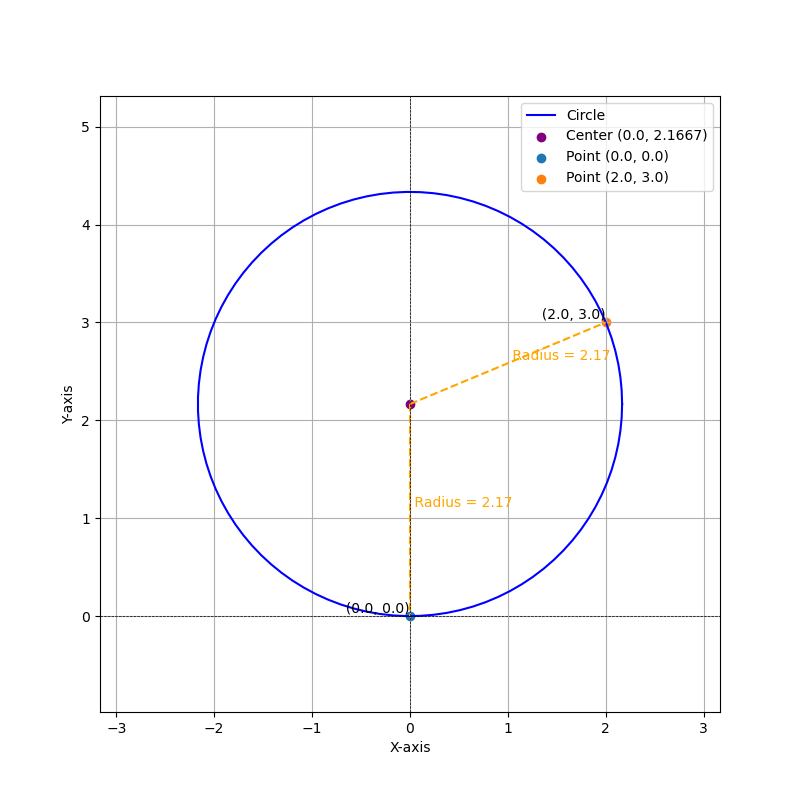
\includegraphics[width=0.7\linewidth]{figs/Fig1.png}
\end{figure}
\end{document}
